
%%% Local Variables:
%%% mode: latex
%%% TeX-master: t
%%% End:
\section{数据在业务中的应用案例}

\subsection{常规交通指标分析}

\begin{frame}[t]{\subsecname}
  \begin{itemize}
     \item<1->出租车
        \begin{enumerate}
          \item 客流量分析(乘次、产生量和吸引量统计)
          \item 出行分析(OD矩阵、OD行程时间和出行距离)
          \item 运营分析(空驶比例、路段行程车速)
        \end{enumerate}
     \item<2->定点车流
        \begin{enumerate}
          \item 流量统计
          \item 流量时变分析
          \item 流向分析(各关口每日出入关的总流量)
        \end{enumerate}
     \item<3->常规公交
        \begin{enumerate}
          \item 客流量分析(线路、站点、换乘)
          \item 出行分析(站点OD、出行OD)
          \item 运营分析(车速、发车频率、候车时间)
          \item 可达性分析
          \item 站点覆盖范围分析
        \end{enumerate}
     \item<4->轨道
        \begin{enumerate}
          \item 客流量统计
          \item 出行统计(站点OD、出行OD、OD行程时间、出行距离)
          \item 运营统计(线路拥挤度、站点拥挤度)
        \end{enumerate}
  \end{itemize}
\end{frame}

\begin{frame}[t]{\subsecname}
  \begin{itemize}
     \item<1-> 居民出行调查
        \begin{enumerate}
          \item 人口、就业、年龄、收入等分布
          \item 交通方式和交通目的比例
          \item 分交通方式和交通目的的出行量
          \item 通勤交通分析 
        \end{enumerate}
  \end{itemize}
  \begin{itemize}
     \item<2-> 手机
        \begin{enumerate}
          \item 就业和居住人口分布
          \item 不分交通方式和目的的出行量
          \item 通勤交通分析 
        \end{enumerate}
  \end{itemize}

\only<3>{
\begin{badbox}{多种数据融合使用} 
   当遇到同一指标存在多种数据源都可以计算的情况,针对应用场景选择最合适的数据进行计算
\end{badbox}}
\end{frame}

\subsection{都市圈范围分析}

\begin{frame}[t]{\subsecname}
\begin{itemize}
  \item<1-> 数据:2010和2016年居民出行调查
  \item<2-> 分析指标
\begin{commonbox}{通勤率定义} 
通勤率=区域R至中心区域通勤人数/区域R常住人口
\end{commonbox}

  \item<3-> 解决问题:深圳市城市边界的空间增长与发展规律
\end{itemize}
\end{frame}

\begin{frame}[t]{\subsecname}
\only<1>{
\begin{figure}
  \centering
  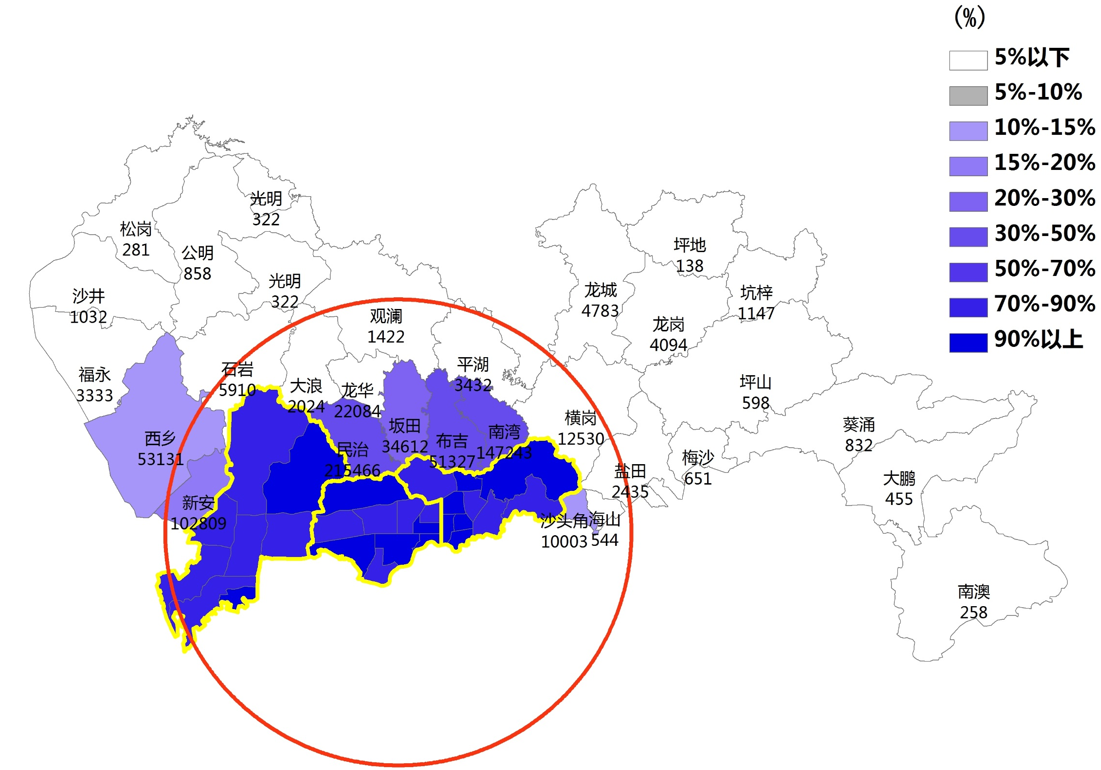
\includegraphics[width=0.9\textwidth]{chp04_中心区2010.png}
  \caption{2010年中心区影响范围(圆心为中心区中心点,圆半径20公里)}
\end{figure}}
\only<2>{
\begin{figure}
  \centering
  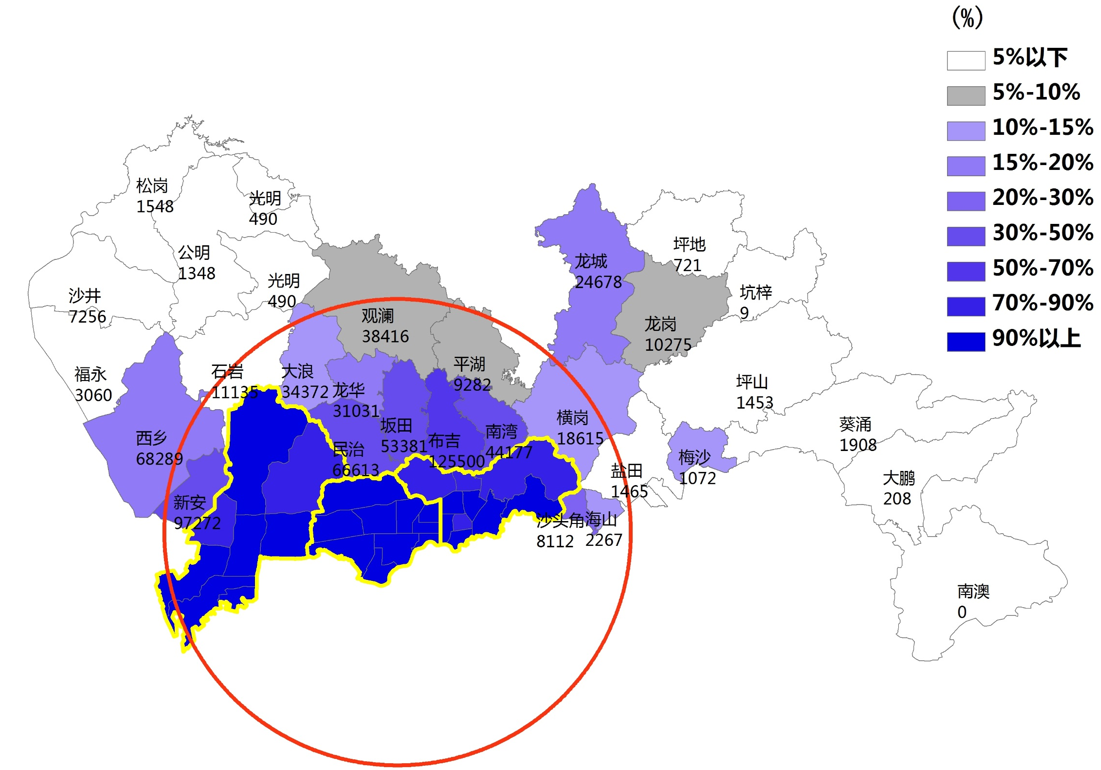
\includegraphics[width=0.9\textwidth]{chp04_中心区2016.png}
  \caption{2016年中心区影响范围(圆心为中心区中心点,圆半径20公里)}
\end{figure}}
\end{frame}

\subsection{区域联系强度分析}
\begin{frame}[t]{\subsecname}
\begin{itemize}
\item 数据:2016年手机数据处理后的交通出行量
\item 解决问题:从交通出行角度探讨深莞边界区域的联系,以及交通组团的划分
\end{itemize}

\begin{overlayarea}{\textwidth}{\textheight}
\vspace{5pt}
  \begin{onlyenv}<2>
\begin{figure}
  \centering
  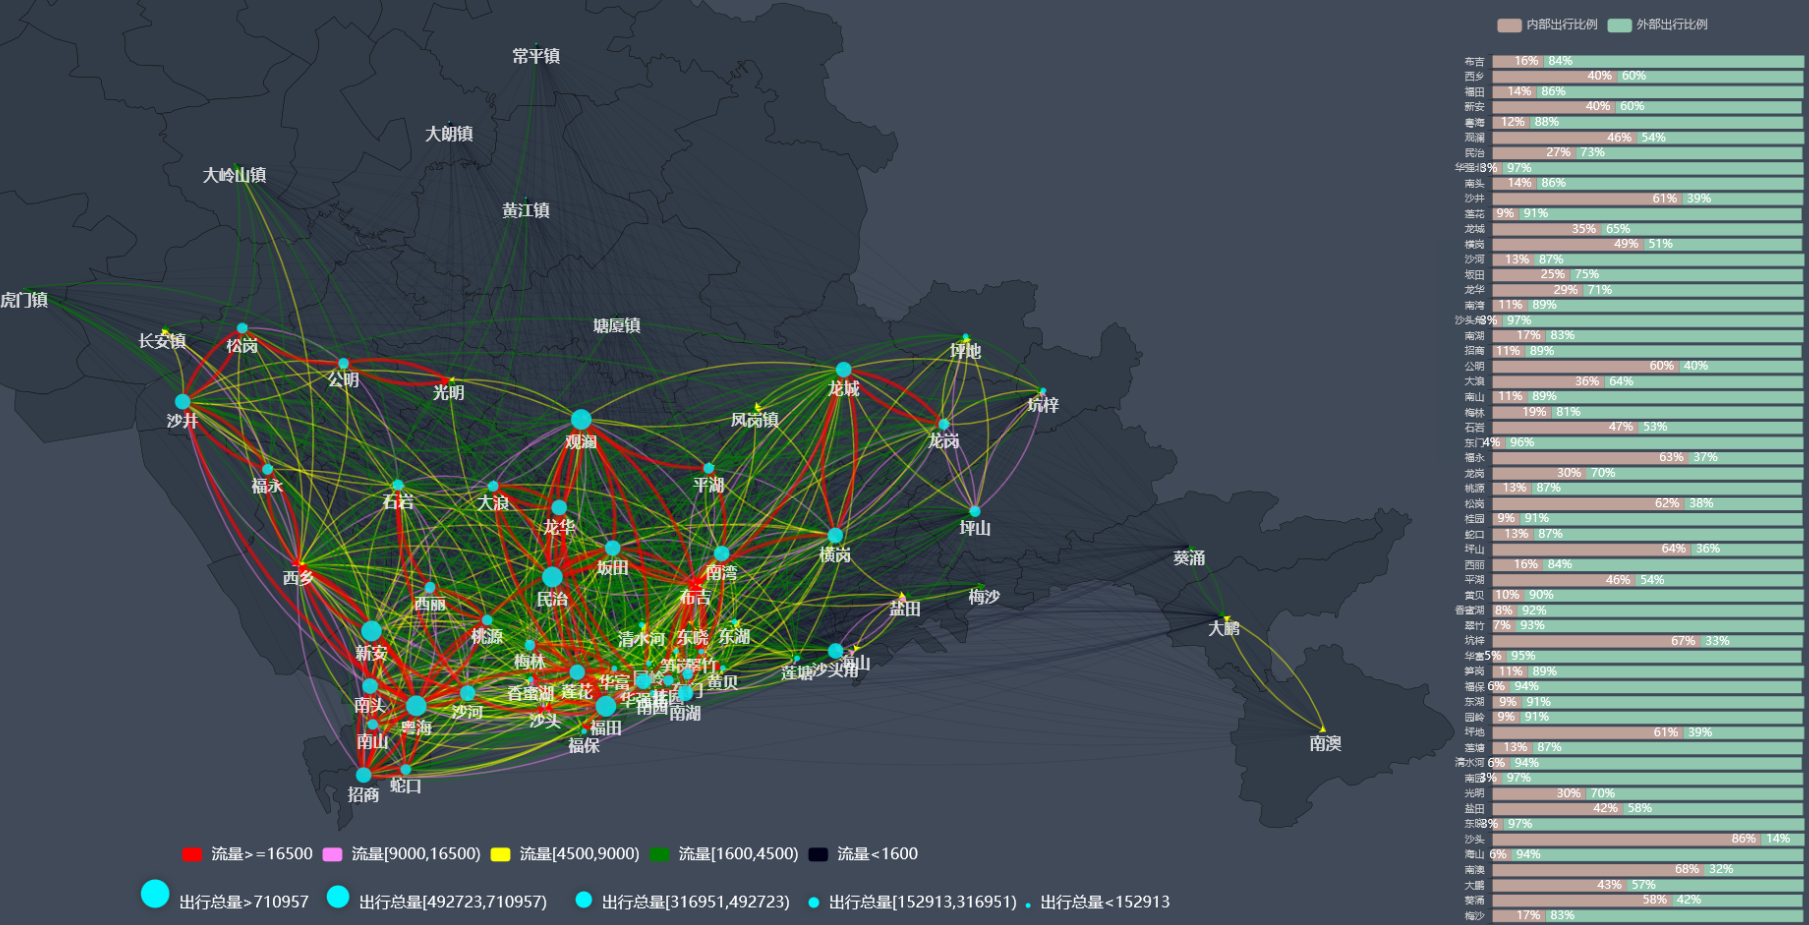
\includegraphics[width=\textwidth]{chp04_深莞出行.png}
  \caption{深莞交通出行}
\end{figure}
  \end{onlyenv}
\end{overlayarea}
\end{frame}

\begin{frame}[t]{\subsecname}
\begin{itemize}
\item<1-> 网络分析中的社区发现(Community Detection)算法
\item<3-> 分析指标:模块度(Modularity)
\end{itemize}

\only<1>{
\begin{figure}
\begin{columns}
  \begin{column}{.6\textwidth}
    \begin{figure}\flushright
      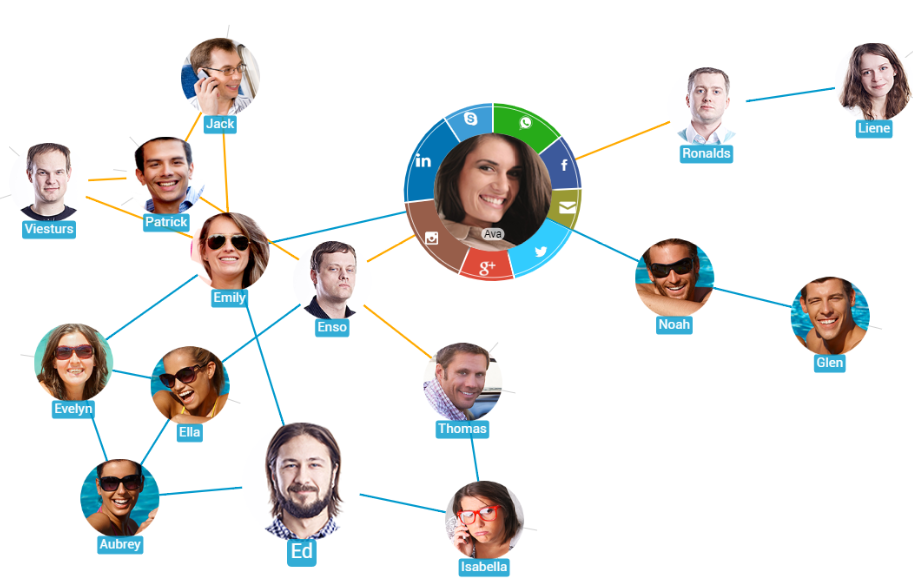
\includegraphics[height=0.4\textheight]{chp04_社交网络1.png}
    \end{figure}
  \end{column}
  \begin{column}{.4\textwidth}
    \begin{figure}\flushleft
      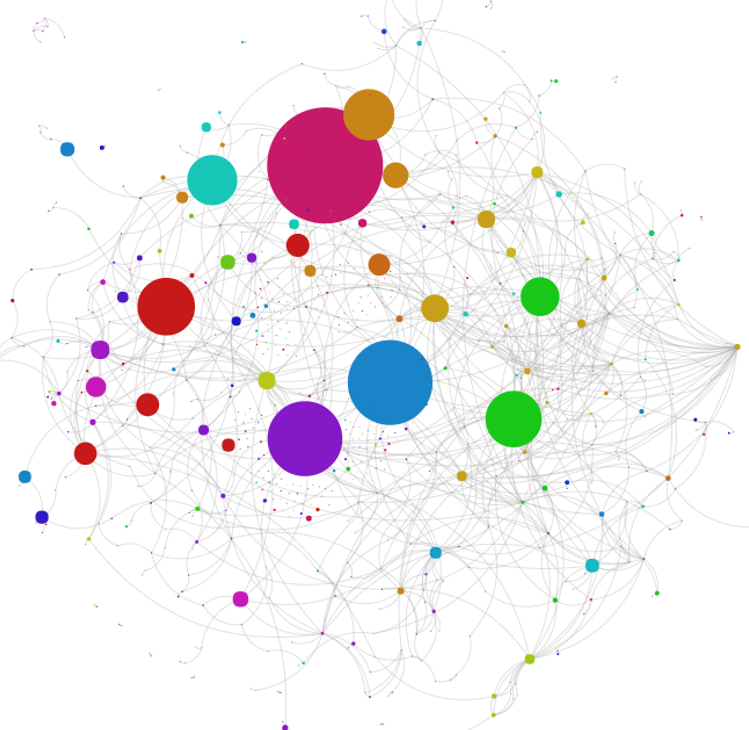
\includegraphics[height=0.4\textheight]{chp04_社交网络2.png}
    \end{figure}
  \end{column}
\end{columns}
\caption{社交网络与网络分析算法}
\end{figure}}

\only<2>{
\begin{badbox}{} 
社区划分的目标是使得划分后的社区内部的连接较为紧密,而在社区之间的连接较为稀疏,网络分析算法中通过\emphText{模块度}指标可以刻画这样的划分的优劣,模块度越大,则社区划分的效果越好
\end{badbox}}

\only<3>{
\begin{commonbox}{模块度定义{\footnotemark[1]}} \footnotesize
网络中连接社区结构内部顶点的边占的比例与另一个随机网络中连接社区结构内部顶点的边所占比例的期望值的差值.
\begin{equation*}
%\mbox{\footnotesize \( Q=\frac{1}{2m}\sum_{ij}\left[ A_{i,j}-\frac{k_ik_j}{2m}\right]\delta(s_i,s_j)\)}
Q=\frac{1}{2m}\sum\nolimits_{i,j}\left[ \omega_{i,j}-\frac{k_ik_j}{2m}\right]\delta(c_i,c_j)=\sum\nolimits_s\left[ \frac{\sum_{in}}{2m}-\left(\frac{\sum_{tot}}{2m} \right)^2\right]
\end{equation*}
其中,${m=\frac{1}{2}\sum\nolimits_{i,j}\omega_{i,j}}$表示网络中所有边的权重之和,$\omega_{i,j}$表示节点$i$和节点$j$之间的权重;$k_i=\sum_j\omega_{i,j}$
表示与顶点$i$连接的所有边的权重;$c$表示的是顶点被分配到的社区,$\delta(s_i,s_j)$用于判断节点$i$与节点$j$是否被划分在同一个社区中,若是则返回1,否则返回0\\
$\sum_{in}$表示社区$c$内部的权重之和,$\sum_{tot}$表示的是与社区$c$内部所有点的连接边的权重之和(包括社区内部的边和社区外部的边)
\end{commonbox}

\footnotetext[1]{\tiny M.E.J. Newman and M.Girvan. 2004. Finding and evaluating community structure in networks[J]. Phys. Rev. E 69, 026113.}}

\vspace{-5pt}
\only<4>{
\begin{algorithm}[H] \tiny
     \SetKwInOut{Input}{输入}
     \SetKwInOut{Output}{输出}
     %\DontPrintSemicolon 
     \caption*{FastUnfolding算法{\footnotemark[1]}}
     \Input{图$G=\{V,E,\omega \}$,节点$V$的数目是$m$,边$E$的数目是$n$,$\omega$是节点之间的权重}
     \Output{分类后的社区集合$\mathbb{C}=\{c_1,c_2,...,c_k\}$}
     \BlankLine    
           
     \lFor{i $\in$ V}{$\mathbb{C}.add(c_i)$\tcc*[r]{把每个节点初始化到不同的社区}}
  
     $best\_gain\leftarrow 0$\tcc*[c]{最优模块度增益}
     $token\leftarrow 0$\tcc*[c]{判断节点是否发生了变化}
     \While{$true$}{
     \For{i $\in$ V}{
        $\mathbb{C}.remove(c_i)$\;
\tcc{计算将节点$i$合并到邻接节点$j$所属社区$c_j$后的模块度增益$\Delta Q$}
        \For{j $\in$ neighbor of i}{   
          $c = \mathbb{C}[j]$\;        
          \If(\tcc*[f]{根据最大增益寻找最合适的社区}){$\Delta Q > best\_gain$}{
             $best\_gain \leftarrow \Delta Q$\;
             $best\_community\leftarrow c$\;  
          }
        $\mathbb{C}.add(best\_community)$\;
       }
       \lIf{$c_i\neq best\_community$}{$token=1$} 
     }
     \lIf{$token=0$}{\textbf{break}} 
}
             
\end{algorithm}
\vspace{5pt}
\footnotetext[1]{\tiny V.D. Blondel, J.L. Guillaume, R. Lambiotte, E. Lefebvre. 2008. Fast unfolding of communities in large networks[J]. J. Stat. Mech: Theory Exp.}}
\end{frame}

\begin{frame}[c]{\subsecname}
\only<1>{
\begin{figure}
  \centering
  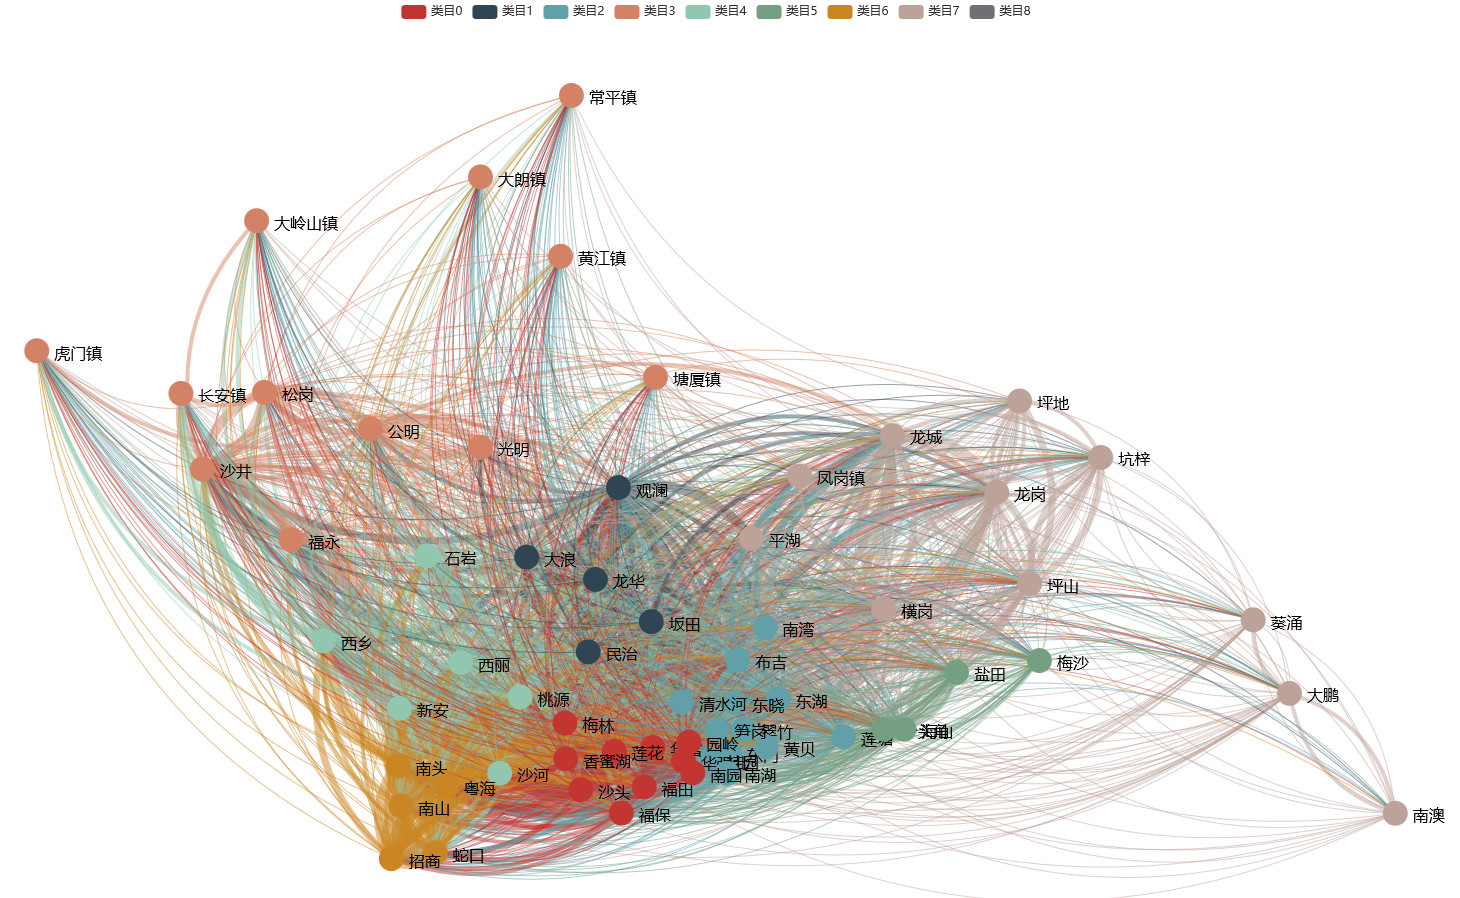
\includegraphics[width=\textwidth]{chp04_社区发现结果2.jpg}
  \caption{基于交通出行联系的社区发现算法实现}
\end{figure}}

\only<2>{
\begin{figure}
  \centering
  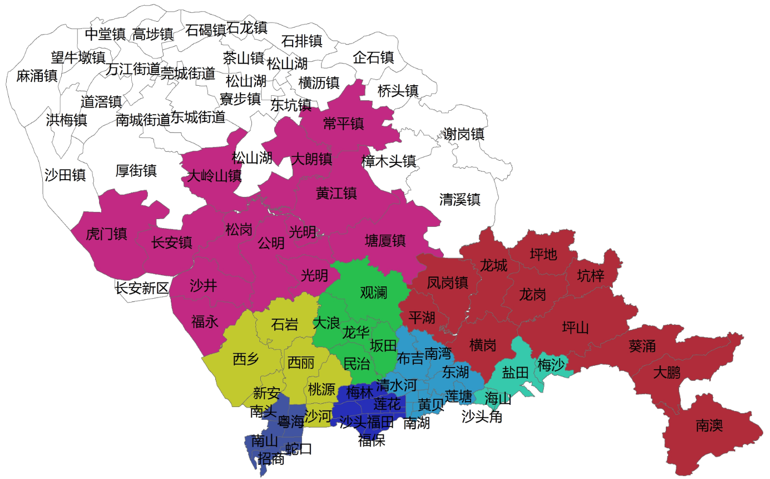
\includegraphics[width=\textwidth]{chp04_社区发现结果3.png}
  \caption{深圳与东莞的新组团范围(不同颜色表示模块度最大的社区)}
\end{figure}}
\end{frame}


\subsection{货运交通分析}
\begin{frame}[t]{\subsecname}
\begin{itemize}
\item 数据:货车GPS数据
\item 解决问题:深圳市对内和对外货运交通的联系 
\end{itemize}

\begin{overlayarea}{\textwidth}{\textheight}
  \begin{onlyenv}<2>
\begin{figure}
  \centering
  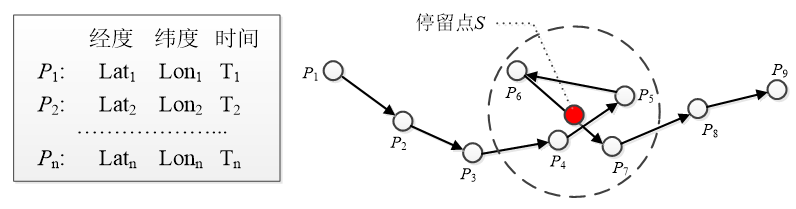
\includegraphics[width=0.8\textwidth]{chp03_停靠点提取算法.png} \\
  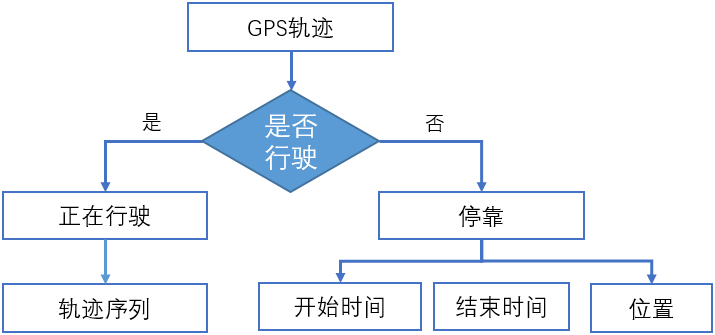
\includegraphics[width=0.6\textwidth]{chp03_GPS轨迹模型.png}
  \caption{车辆轨迹模型}
\end{figure}
  \end{onlyenv}

  \begin{onlyenv}<3>
\begin{algorithm}[H] \tiny
     \SetKwInOut{Input}{输入}
     \SetKwInOut{Output}{输出}
     %\DontPrintSemicolon 
     \caption*{停留位置识别}
     \Input{GPS点序列$P$,距离阈值$distThreh$,时间阈值$timeThreh$}
     \Output{停留点集合$SP$=\{$S$\}}
     \BlankLine    
     $i=0; pointNum=\left| P \right|$\;
     \While{$i<pointNum$}{$j \leftarrow i+1; Label=0$\;
     \While{$j<pointNum$}{
     $dist$=Distance($p_i$,$p_j$)\tcc*[r]{计算两点距离}
     \If{$dist>distThreh$}{$\Delta T\leftarrow p_j.T-p_i.T$\tcc*[r]{计算两点时间差}
     \If{$\Delta T>timeThreh$}{
      $S.coord \leftarrow$ ComputeMeanCoord({$p_k|i\leqslant k\leqslant j$})\tcc*[r]{计算静止点集的中心坐标}
      $S.arvT \leftarrow p_i.T; S.levT \leftarrow p_j.T$\;
      $SP.insert(S)$\;
      $i\leftarrow j;Label\leftarrow 1$\;}
      \textbf{break}\;}
      $j=j+1$\;}
      \lIf{$Label\neq 1$}{$i=i+1$}}
      \Return $SP$\;                 
\end{algorithm}
  \end{onlyenv}

\vspace{-10pt}
  \begin{onlyenv}<4>
\begin{figure}
  \centering
  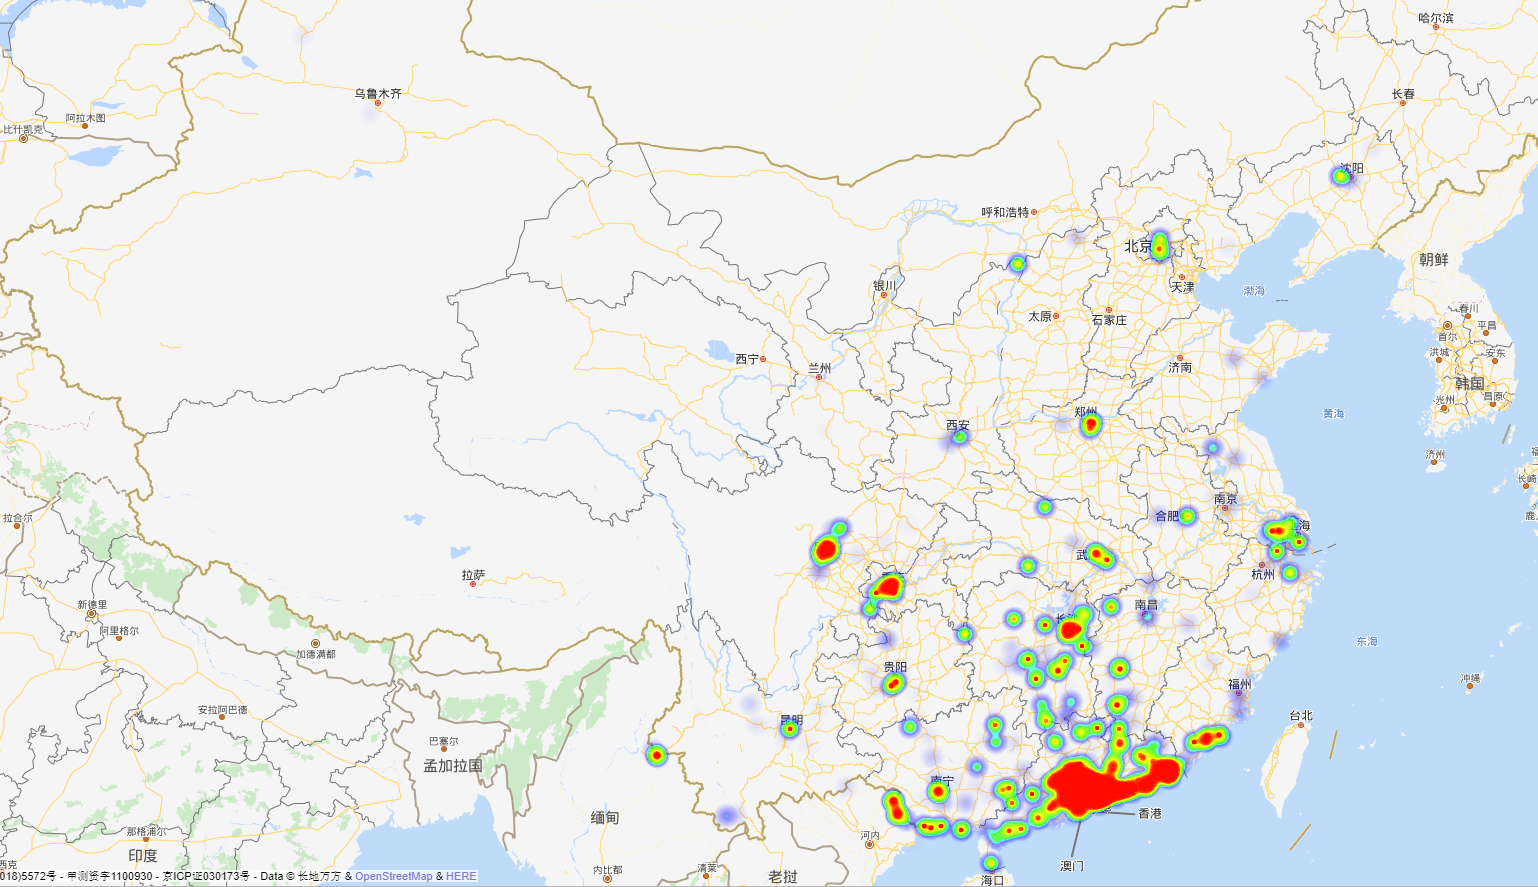
\includegraphics[width=0.9\textwidth]{chp04_货车全国停靠点.png}
  \caption{深圳市货车在全国的货场分布}
\end{figure}
  \end{onlyenv}

  \begin{onlyenv}<5>
\begin{figure}
  \centering
  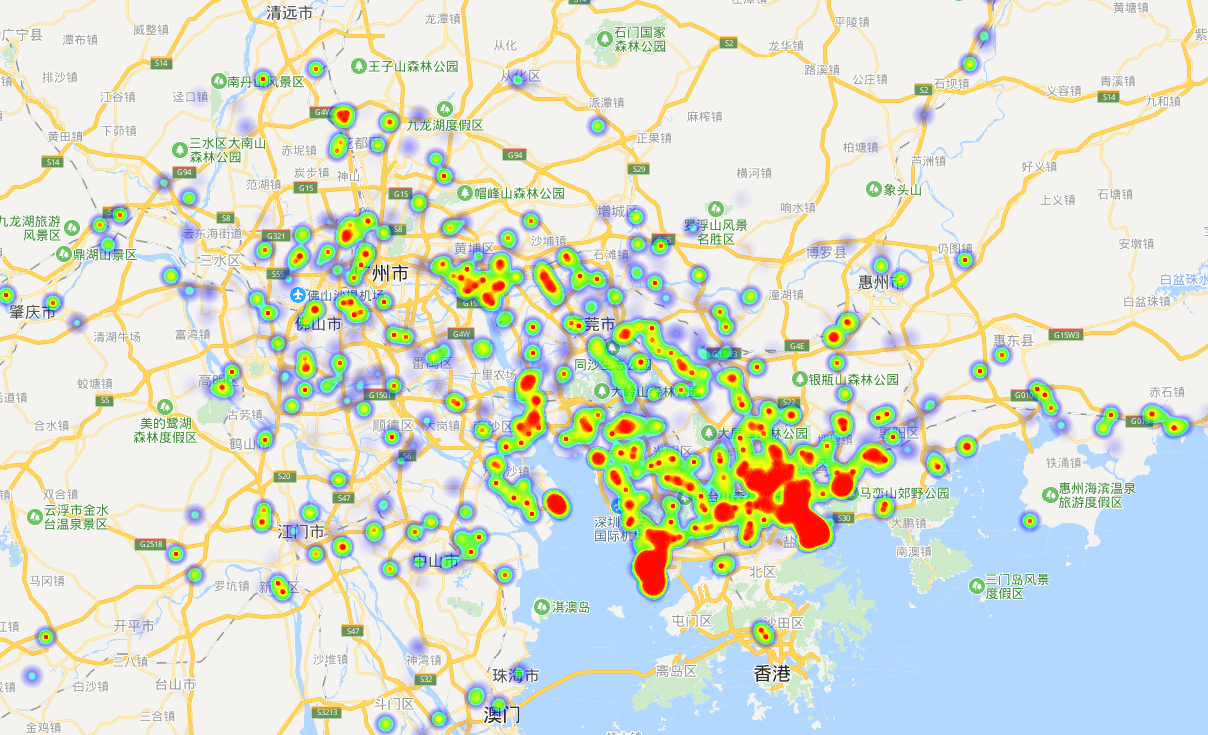
\includegraphics[width=0.9\textwidth]{chp04_货车珠三角停靠点.png}
  \caption{深圳市货车在珠三角的货场分布}
\end{figure}
  \end{onlyenv}

  \begin{onlyenv}<6>
\begin{figure}
  \centering
  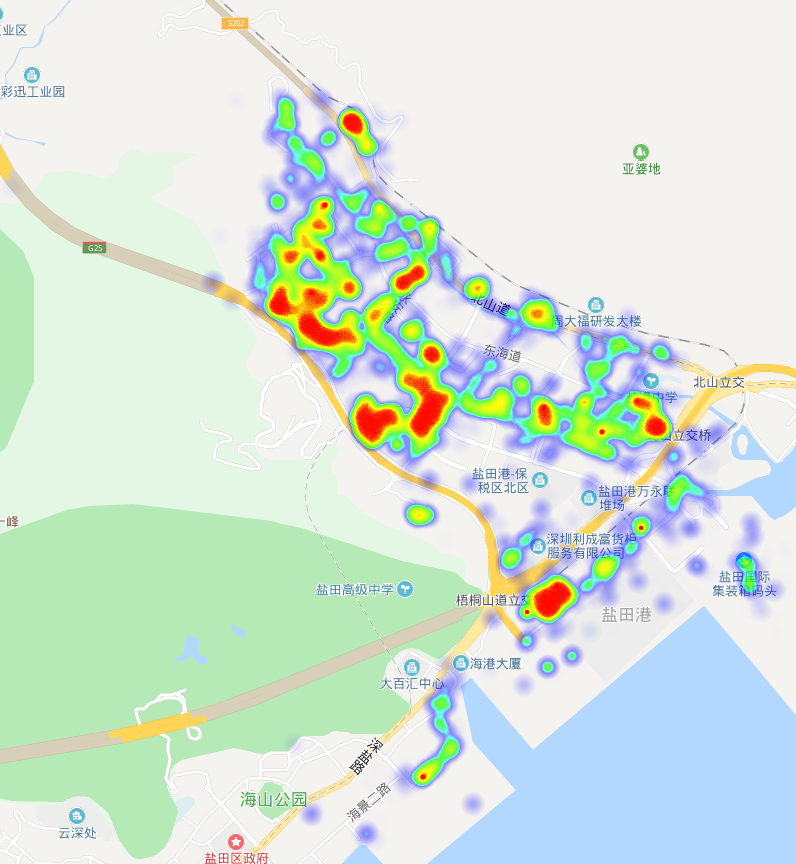
\includegraphics[width=0.5\textwidth]{chp04_货车盐田港停靠点.png}
  \caption{深圳市货车在盐田港区的货场分布}
\end{figure}
  \end{onlyenv}

  \begin{onlyenv}<7>
\begin{figure}
  \centering
  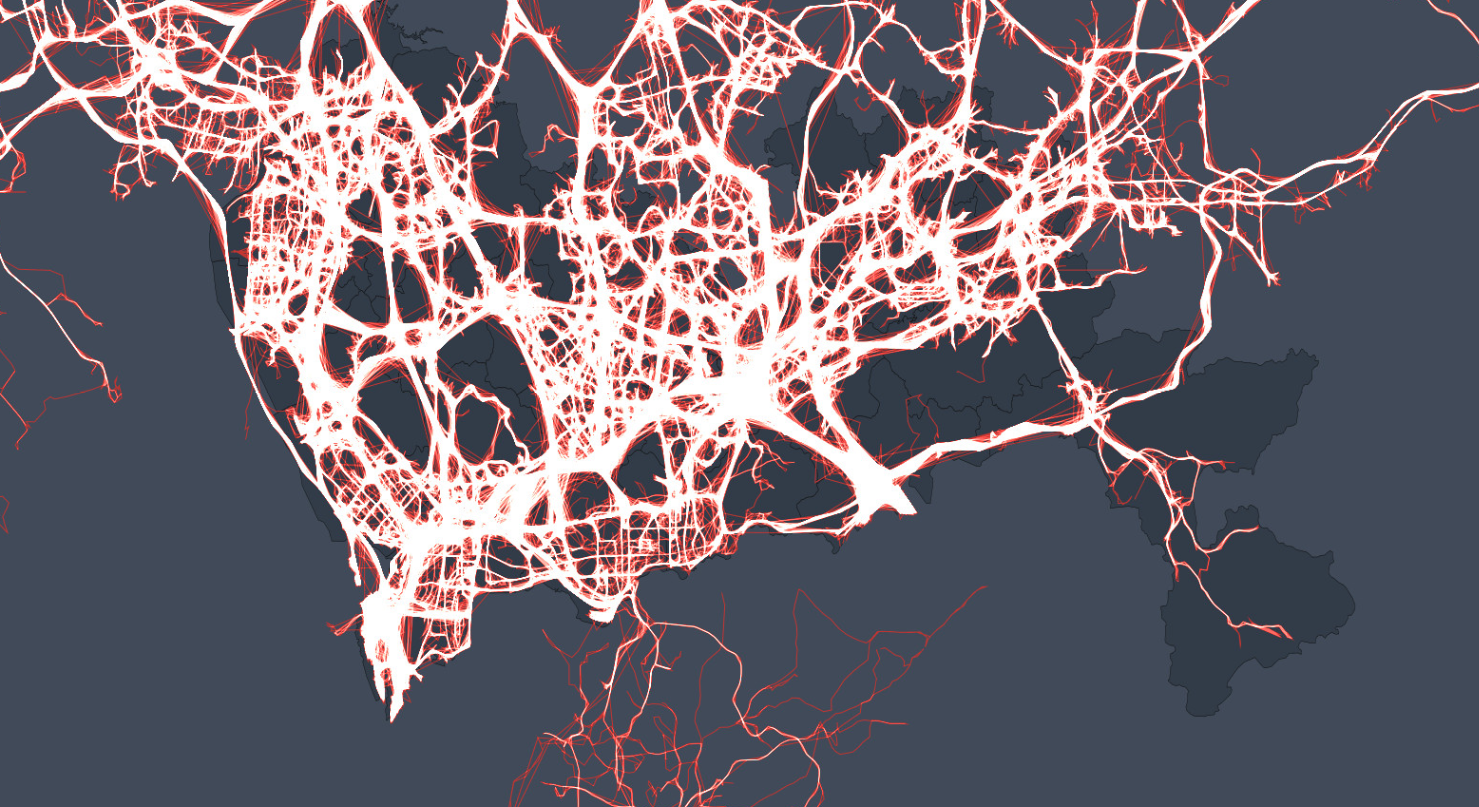
\includegraphics[width=\textwidth]{chp04_车辆轨迹地图.png}
  \caption{车辆轨迹地图}
\end{figure}
  \end{onlyenv}

  \begin{onlyenv}<8>
\begin{figure}
  \centering
  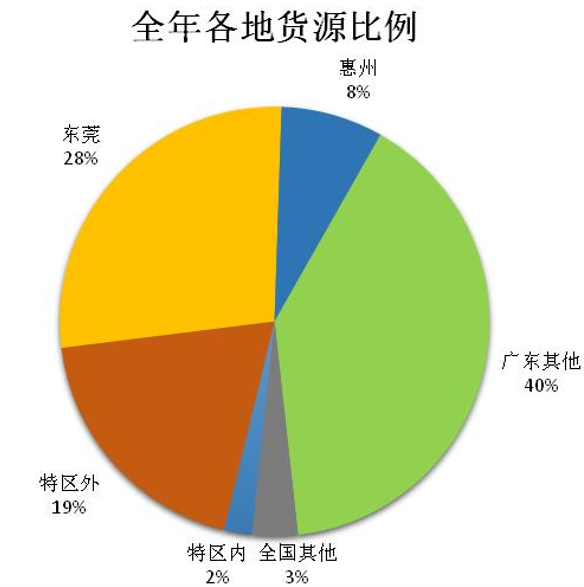
\includegraphics[width=0.5\textwidth]{chp04_货源地分布.png}
  \caption{除了空间表达形式之外,还可以分析各类统计指标}
\end{figure}
  \end{onlyenv}

  \begin{onlyenv}<9>
\begin{figure}
  \centering
  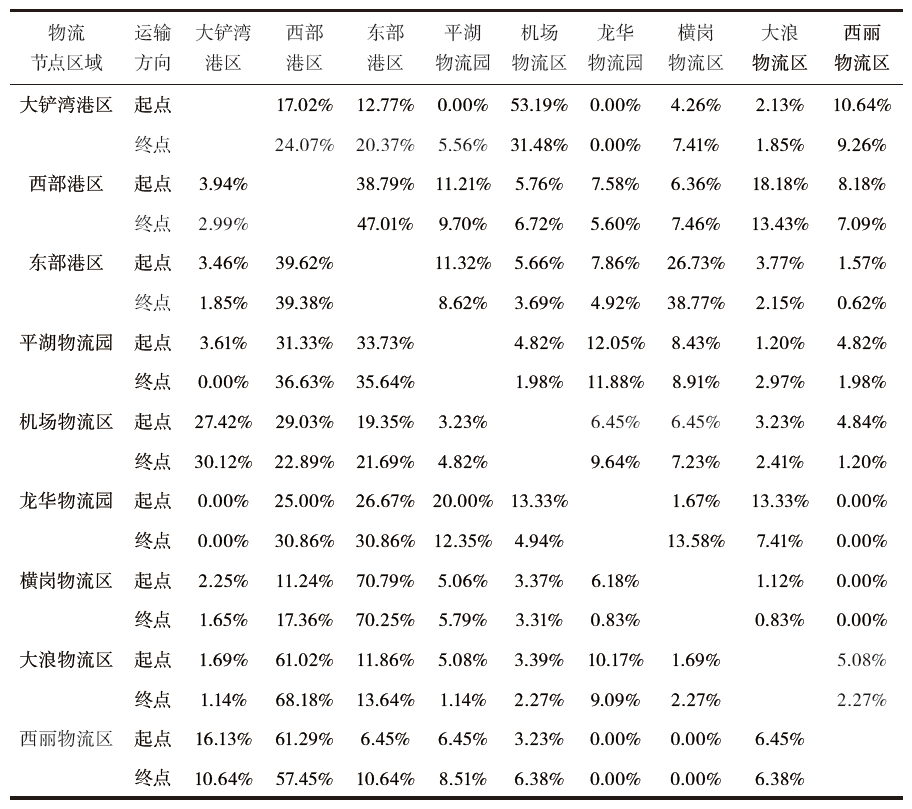
\includegraphics[width=0.6\textwidth]{chp04_货运分析结果.png}
  \caption{除了空间表达形式之外,还可以分析各类统计指标}
\end{figure}
  \end{onlyenv}
\end{overlayarea}
\end{frame}



